%!TeX spellcheck = en-GB

\documentclass[hyperref={colorlinks=true,urlcolor=blue,linkcolor=.},aspectratio=1610,mathserif]{beamer}
\usepackage[utf8]{inputenc}
\usepackage{pgfpages}
\usepackage{graphicx}
\usepackage{pdfpages}
\usepackage{tikz}
\usepackage[many]{tcolorbox}
\usepackage[autoplay,loop,keepaspectratio]{animate}
\usepackage{siunitx}
\sisetup{
	per-mode = symbol,
	round-mode = figures,
	round-precision = 3,
	scientific-notation = false,
	output-decimal-marker = {.},
	exponent-product = \times,
	separate-uncertainty = true,
	uncertainty-separator = ,
	output-product = \cdot,
	quotient-mode = fraction,
	range-phrase = -,
	range-units = single,
	inter-unit-product = \ensuremath{{\cdot{}}},
	number-unit-product = \,,
	multi-part-units = single,
	alsoload = synchem,
}
\DeclareSIUnit\atm{atm}
\usepackage{nth}
\usepackage{physics}

% ------------------------ Define note handout layout -------------------------
\newcommand{\pgflayout}{
	\pgfpagesphysicalpageoptions
	{%
		logical pages=2,%
		physical height=210mm,%
		physical width=297mm,%
	}%
	\pgfpageslogicalpageoptions{2}
	{%
		resized width=\pgfphysicalwidth,%
		resized height=\pgfphysicalheight,%
		center=\pgfpoint{.5\pgfphysicalwidth}{.25\pgfphysicalheight}%
	}%
	\pgfpageslogicalpageoptions{1}
	{%
		resized width=\pgfphysicalwidth,%
		resized height=\pgfphysicalheight,%
		center=\pgfpoint{.5\pgfphysicalwidth}{.70\pgfphysicalheight}%
	}%
}
% -----------------------------------------------------------------------------

% ---------------------------- Show note handout: -----------------------------
%\setbeameroption{show only notes}
%\pgflayout
% -----------------------------------------------------------------------------

% -------------------------- Define Beamer options ----------------------------
\beamertemplatenavigationsymbolsempty
\usefonttheme{structuresmallcapsserif}
\usecolortheme{beaver}

\setbeamertemplate{footline}
{%
	\begin{beamercolorbox}{section in foot}
		\begin{center}
			\vskip2pt\insertnavigation{\paperwidth}\vskip2pt
		\end{center}
	\end{beamercolorbox}%
}

\setbeamertemplate{note page}{%
	\vskip7em
	\begin{columns}[c]{\paperheight}
		\column{0.5\paperheight}
		\insertnote
		\column{0.5\paperheight}
		\insertslideintonotes{0.5}
	\end{columns}%
}

\setbeamersize{text margin left=30mm,text margin right=30mm}

\definecolor{DTUred}{cmyk}{0,0.91,0.72,0.23}
\definecolor{itemcolor}{cmyk}{0,0,0,0.56}
\definecolor{blockbodycolor}{cmyk}{0,1,1,0.5}
\definecolor{White}{cmyk}{0,0,0,0}
\setbeamercolor{titlelike}{fg=DTUred}
\setbeamercolor{section in head/foot}{fg=DTUred}
\setbeamercolor{section in toc}{fg=DTUred}
\setbeamercolor{itemize item}{fg=itemcolor}
\setbeamercolor{redbox}{fg=White,bg=blockbodycolor}
\setbeamercolor{description item}{fg=DTUred}
% -----------------------------------------------------------------------------

\title{Assignment 1 \& 2}
\subtitle{Course 10401}
\author{\scshape\centering Nicklas Kihm (s143286) \\ Rasmus Kronborg Finnemann Wiuff (s163977) \\ \vspace{7.5mm} 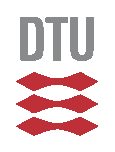
\includegraphics[width=1cm]{Figures/DTU3CMYK.eps}}
\date{\scshape January 17, 2019}

\begin{document}

\begin{frame}[plain]
	\titlepage
\end{frame}

\section{Introduction}
\subsection{Introduction}
\begin{frame}
	\frametitle{Introduction}
	\begin{center}
		\textbf{Assignment 1} \hspace{5cm} \textbf{Assignment 2}
		\begin{columns}[c]
			\column{.7\textwidth}
			\begin{description}[Goal \# 1]
				\item[Title] Fusion power plant
				\item[Goal] Design a tokamak using a modified version of the model presented in Freidberg's book.
			\end{description}
			\vskip1.5em
			\column{.7\textwidth}
			\begin{description}[Goal \# 1]
				\item[Title] Design of interferometer for DTU tokamak
				\item[Goal \# 1] To calculate the phase shift induced by O-mode radiation and investigate different microwave sources
				\item[Goal \# 2] To design a lens system to accommodate the beam propagation in the small DTU tokamak
			\end{description}
		\end{columns}
	\end{center}
\end{frame}


\section{Fusion power plant}
\subsection{Fusion power plant}
\begin{frame}
	\frametitle{Fusion power plant- Freidberg's model}
	\centering
	\begin{beamercolorbox}[sep=1em,wd=8cm]{redbox}
		Freidberg assumes a circular plasma cross section. Output parameters presented in the textbook are calculated given a few input parameters.
	\end{beamercolorbox}
\end{frame}
\begin{frame}
	\frametitle{Input parameters}
	\centering
	\begin{table}
		\begin{tabular}{lrl}
			Symbol                         & Quantity                                      &                                              \\
			\(n_\mathrm{flux \ fraction}\) & n flux in breeder end/n flux in breeder start & \(\bqty{}\)                                  \\
			\(C_F\)                        & Fixed cost propotionality constant            & \(\bqty{\$}\)                                \\
			\(C_I\)                        & Nuclear island cost propotionality constant   & \(\bqty{\$\cdot\si{\watt\per\meter\cubed}}\) \\
			\(P_E\)                        & Desired output power                          & \(\bqty{\si{\mega\watt}}\)                   \\
			\(P_W\)                        & Maximum wall load                             & \(\bqty{\si{\mega\watt\per\meter\squared}}\) \\
			\(B_{\max}\)                   & Magnetic field at the edge of the coil        & \(\bqty{\si{\tesla}}\)                       \\
			\(\sigma_{\max}\)              & Tensile strenght of the magnetic field coils  & \(\bqty{\si{\atm}}\)                         \\
			\(\eta_t\)                     & Energy conversion efficiency                  & \(\bqty{}\)                                  \\
		\end{tabular}
	\end{table}
\end{frame}
\begin{frame}{Output parameters}
	\centering
	\begin{table}
		\begin{tabular}{llrl}
			Symbol              & Quantity                                               & Obtained values &                       \\
			\(b\)               & Blanket-and-shield thickness                           & 1.2037          & \si{\meter}           \\
			\(c\)               & Magnet coil thickness                                  & 0.7993          & \si{\meter}           \\
			\(a\)               & Minor radius                                           & 2.0098          & \si{\meter}           \\
			\(R_0\)             & Major radius                                           & 4.9583          & \si{\meter}           \\
			\(A\)               & Aspect ratio                                           & 2.4670          & \(\bqty{}\)           \\
			\(A_p\)             & Plasma surface                                         & 393.4152        & \si{\meter\squared}   \\
			\(V_p\)             & Plasma volume                                          & 395.3509        & \si{\meter\cubed}     \\
			\(P_\mathrm{dens}\) & Power density                                          & 4.9685e06       & \si{\watt\per\meter}  \\
			\(p\)               & Plasma pressure                                        & 7.3672e05       & \si{\pascal}          \\
			\(n\)               & Particle density                                       & 1.5327e20       & \si{\per\meter\cubed} \\
			\(B_0\)             & Magnetic field at magnetic axis                        & 4.5744          & \si{\tesla}           \\
			\(\beta\)           & Normalised plasma pressure                             & 8.85            & \(\%\)                \\
			\(\tau_{E_\min}\)   & Min confinement time for \(\pqty{p\times\tau_E}_\min\) & 1.1415          & \si{\second}          \\
		\end{tabular}
	\end{table}
\end{frame}
\begin{frame}
	\frametitle{Model sensitivity}
	\begin{columns}
		\column[c]{.5\textwidth}
		\begin{centering}
			\begin{beamercolorbox}[sep=1em,wd=8cm]{redbox}
				\(P_{\si{E}}\), \(P_{\si{W}}\), \(B_{\max}\) and \(\sigma_{\max}\) are changed. Many output parameters were unaffected or changed linearly. But some interesting results were found.
			\end{beamercolorbox}
		\end{centering}
		\column[c]{.5\textwidth}
		\centering
		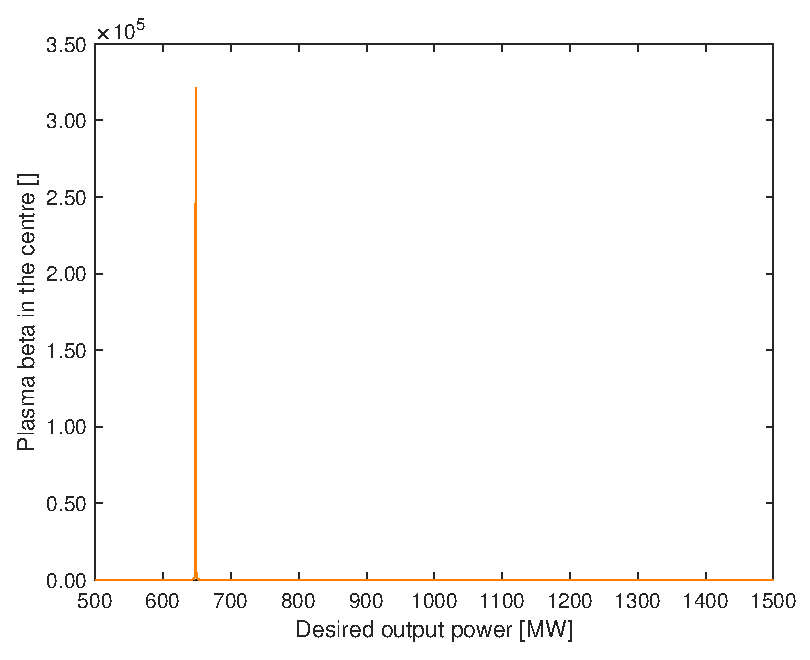
\includegraphics[width=\textwidth]{MatlabFigures/DesiredOutputPower/PlasmaBetaInTheCentre.eps}
		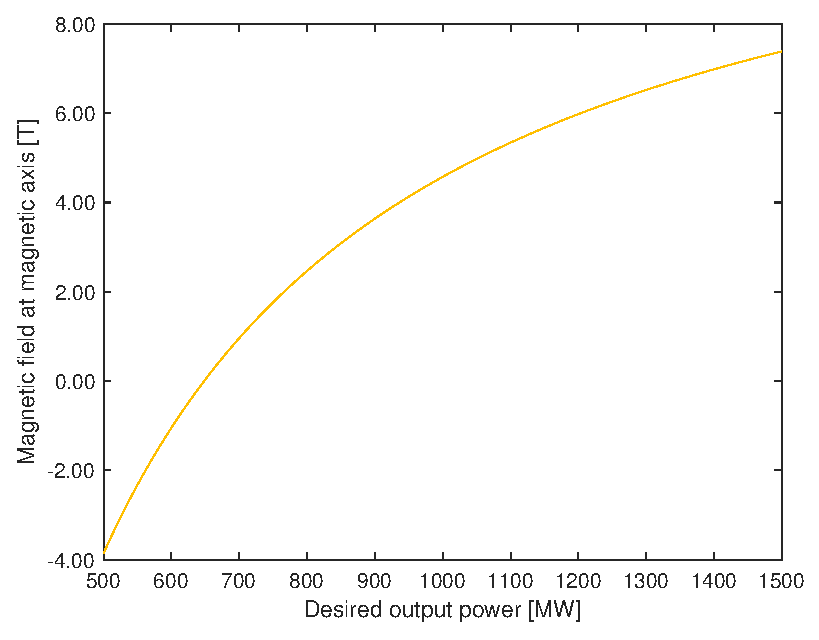
\includegraphics[width=\textwidth]{MatlabFigures/DesiredOutputPower/MagneticFieldAtMagneticAxis.eps}
	\end{columns}
\end{frame}

\begin{frame}
	\frametitle{Elliptic plasma-changes in model}
	\begin{columns}
		\column[c]{.5\textwidth}
		\begin{beamercolorbox}[sep=1em,wd=8cm]{redbox}
			Now the plasma is modeled as an ellipse.
			The thickness of the blanket is not constant. Rather the outer and inner ellipses are kept as true ellipses.
		\end{beamercolorbox}
		\begin{align}
			V_{\si{I}}=2\,\pi^{2}\, R_{0}\,((a_{\min}+b+c)^{2}-a_{\min}^{2})\,\kappa
		\end{align}
		\begin{align}
			c=\frac{2\,\xi}{1-\xi}\,(\kappa\, a_{\min}+b)
		\end{align}
		\column[c]{.6\textwidth}
		\centering
		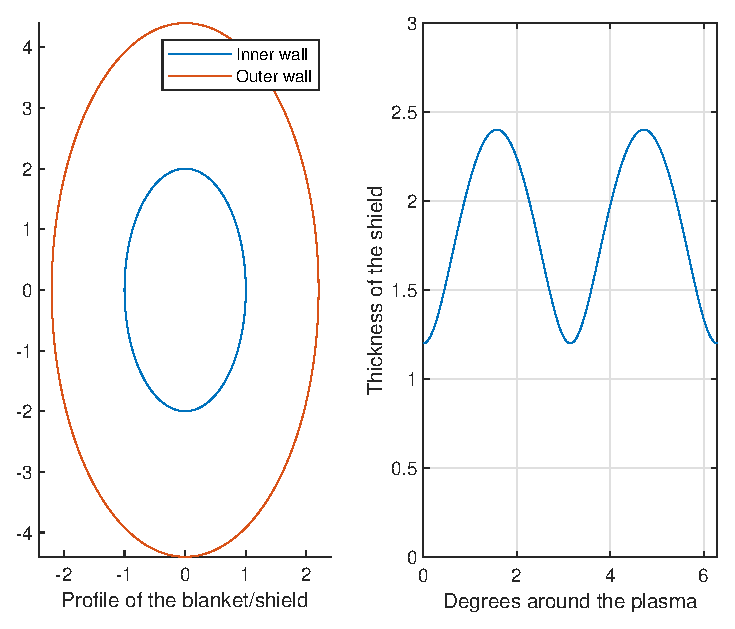
\includegraphics[width=\textwidth]{MatlabFigures/ShieldThickness/ShieldThickness.eps}
	\end{columns}
\end{frame}

\begin{frame}
	\frametitle{Elliptical model output parameters}
	\centering
	\begin{table}
		\begin{tabular}{llr}
			Symbol              & Quantity                                               & Obtained values                          \\
			\(c\)               & Magnet coil thickness                                  & \SI{1.30}{\meter}\uparrow                \\
			\(A_p\)             & Plasma surface                                         & \SI{1206}{\meter\squared}\uparrow        \\
			\(V_p\)             & Plasma volume                                          & \SI{793}{\meter\cubed}\uparrow           \\
			\(P_\mathrm{dens}\) & Power density                                          & \SI{2.48e06}{\watt\per\meter}\downarrow  \\
			\(p\)               & Plasma pressure                                        & \SI{5.20e05}{\pascal}\downarrow          \\
			\(n\)               & Particle density                                       & \SI{1.08e20}{\per\meter\cubed}\downarrow \\
			\(\beta\)           & Normalised plasma pressure                             & 6.17\%\downarrow                         \\
			\(\tau_{E_\min}\)   & Min confinement time for \(\pqty{p\times\tau_E}_\min\) & \SI{1.62}{\second}\uparrow               \\
		\end{tabular}
	\end{table}
\end{frame}

\begin{frame}
	\frametitle{DEMO output parameters with \(P_{\si}=2GW\)}
	\centering
	\begin{table}
		\begin{tabular}{llr}
			Symbol              & Quantity                                               & Obtained values                      \\
			\(b\)               & Blanket-and-shield thickness                           & \SI{1.20}{\meter}                    \\
			\(c\)               & Magnet coil thickness                                  & \SI{1.30}{\meter}                    \\
			\(a\)               & Minor radius                                           & \SI{2.01}{\meter}                    \\
			\(R_0\)             & Major radius                                           & \SI{9.95}{\meter}\uparrow            \\
			\(A\)               & Aspect ratio                                           & 4.95\uparrow                         \\
			\(A_p\)             & Plasma surface                                         & \SI{2.41e03}{\meter\squared}\uparrow \\
			\(V_p\)             & Plasma volume                                          & \SI{1.59e03}{\meter\cubed}\uparrow   \\
			\(P_\mathrm{dens}\) & Power density                                          & \SI{2.48e06}{\watt\per\meter}        \\
			\(p\)               & Plasma pressure                                        & \SI{5.20e05}{\pascal}                \\
			\(n\)               & Particle density                                       & \SI{1.08e20}{\per\meter\cubed}       \\
			\(B_0\)             & Magnetic field at magnetic axis                        & \SI{8.80}{\tesla}\uparrow            \\
			\(\beta\)           & Normalised plasma pressure                             & 1.69\%\downarrow                     \\
			\(\tau_{E_\min}\)   & Min confinement time for \(\pqty{p\times\tau_E}_\min\) & \SI{1.62}{\second}                   \\
		\end{tabular}
	\end{table}
\end{frame}



\begin{frame}
	\frametitle{DEMO output parameters with \(\kappa=2\) and \(A=3\)}
	\centering
	\begin{table}
		\begin{tabular}{llr}
			Symbol              & Quantity                                               & Obtained values                            \\
			\(b\)               & Blanket-and-shield thickness                           & \SI{1.20}{\meter}                          \\
			\(c\)               & Magnet coil thickness                                  & \SI{1.30}{\meter}                          \\
			\(a\)               & Minor radius                                           & \SI{2.01}{\meter}                          \\
			\(R_0\)             & Major radius                                           & \SI{6.03}{\meter}    \downarrow            \\
			\(A\)               & Aspect ratio                                           & 3       \downarrow                         \\
			\(A_p\)             & Plasma surface                                         & \SI{1.46e03}{\meter\squared}    \downarrow \\
			\(V_p\)             & Plasma volume                                          & \SI{962}{\meter\cubed}    \downarrow       \\
			\(P_\mathrm{dens}\) & Power density                                          & \SI{4.01e06}{\watt\per\meter}  \uparrow    \\
			\(p\)               & Plasma pressure                                        & \SI{6.68e05}{\pascal}    \uparrow          \\
			\(n\)               & Particle density                                       & \SI{1.39e20}{\per\meter\cubed}\uparrow     \\
			\(B_0\)             & Magnetic field at magnetic axis                        & \SI{6.07}{\tesla}   \downarrow             \\
			\(\beta\)           & Normalised plasma pressure                             & 4.55\%    \uparrow                         \\
			\(\tau_{E_\min}\)   & Min confinement time for \(\pqty{p\times\tau_E}_\min\) & \SI{1.26}{\second}     \downarrow          \\
		\end{tabular}
	\end{table}
\end{frame}

\begin{frame}
	\frametitle{DEMO with \(\kappa\) and \(A\) as free parameters}
	\begin{centering}
		\begin{beamercolorbox}[sep=1em,wd=8cm]{redbox}
			We have chosen to optimise the engineering volume and \(\beta\) using \(\kappa\) and \(A\) as free parameters. This yields optimum \(R_{0}\) and \(\kappa\)
		\end{beamercolorbox}
	\end{centering}
	\begin{align}
		R_{0}=\sqrt{a^{3}/b}
	\end{align}
	\begin{align}
		\kappa=\frac{6\, a_{\min}\,\xi-b\,\xi-6\, a_{\min}-b}{2\, a_{\min}\,\xi}
	\end{align}
\end{frame}
\begin{frame}
	\frametitle{DEMO output parameters with \(\kappa\) and \(A\) as free parameters}
	\centering
	\begin{table}
		\begin{tabular}{llr}
			Symbol                      & Quantity                                               & Obtained values                           \\
			\(b\)                       & Blanket-and-shield thickness                           & \SI{1.20}{\meter}                         \\
			\(c\)                       & Magnet coil thickness                                  & \SI{1.30}{\meter}                         \\
			\(a\)                       & Minor radius                                           & \SI{2.01}{\meter}                         \\
			\(R_0\)                     & Major radius                                           & \SI{2.60}{\meter}  \downarrow             \\
			\(A\)                       & Aspect ratio                                           & 1.29           \downarrow                 \\
			\(A_p\)                     & Plasma surface                                         & \SI{630}{\meter\squared}                  \\
			\(V_p\)                     & Plasma volume                                          & \SI{414}{\meter\cubed}    \downarrow      \\
			\(P_\mathrm{dens}\)         & Power density                                          & \SI{9.49e06}{\watt\per\meter} \downarrow  \\
			\(p\)            \downarrow & Plasma pressure                                        & \SI{1.02e05}{\pascal}                     \\
			\(n\)                       & Particle density                                       & \SI{2.12e20}{\per\meter\cubed} \downarrow \\
			\(B_0\)                     & Magnetic field at magnetic axis                        & \SI{-3.09}{\tesla}    \downarrow          \\
			\(\beta\)                   & Normalised plasma pressure                             & 26.9\%     \uparrow                       \\
			\(\tau_{E_\min}\)           & Min confinement time for \(\pqty{p\times\tau_E}_\min\) & \SI{1.26}{\second}                        \\
		\end{tabular}
	\end{table}
\end{frame}


\section{Diagnostic Interferometer}
\subsection{Diagnostic Interferometer}
\begin{frame}{Cut off}
	\begin{align}
		n_e < n_c & = \omega^2\frac{\epsilon_0\cdot m_{e0}}{e^2}
	\end{align}
	\begin{align}
		\omega^2\frac{\epsilon_0\cdot m_{e0}}{e^2} & = \omega^2\frac{\SI{8.854e-12}{\farad\per\meter}\SI{9.109e-31}{\kilo\gram}}{\SI{1.602e-19}{\coulomb}} \\
		                                           & \Downarrow\nonumber                                                                                   \\
		n_e                                        & < 0.000314\omega^2
	\end{align}
	At densities of \SI{e18}{\per\meter\cubed} the minimum frequency is:
	\begin{align}
		\frac{\omega}{2\pi} & > \frac{\sqrt{\frac{\SI{e18}{\per\meter\cubed}}{0.000314}}}{2\pi} \\
		                    & \Downarrow\nonumber                                               \\
		f                   & \approx \SI{9}{\giga\hertz}
	\end{align}
\end{frame}
\begin{frame}{Four Sources}
	\begin{columns}
		\column{.6\textwidth}\\
		At a density of \SI{e18}{\per\meter\cubed} the minimum frequency of the wave is:
		\(f \approx \SI{9}{\giga\hertz}\)\newline
		\begin{itemize}
			\item \SI{2.45}{\giga\hertz} (Transparent)
			\item \SI{60}{\giga\hertz}
			\item \SI{98}{\giga\hertz}
			\item \SI{130}{\giga\hertz}
		\end{itemize}
		\column{.6\textwidth}
		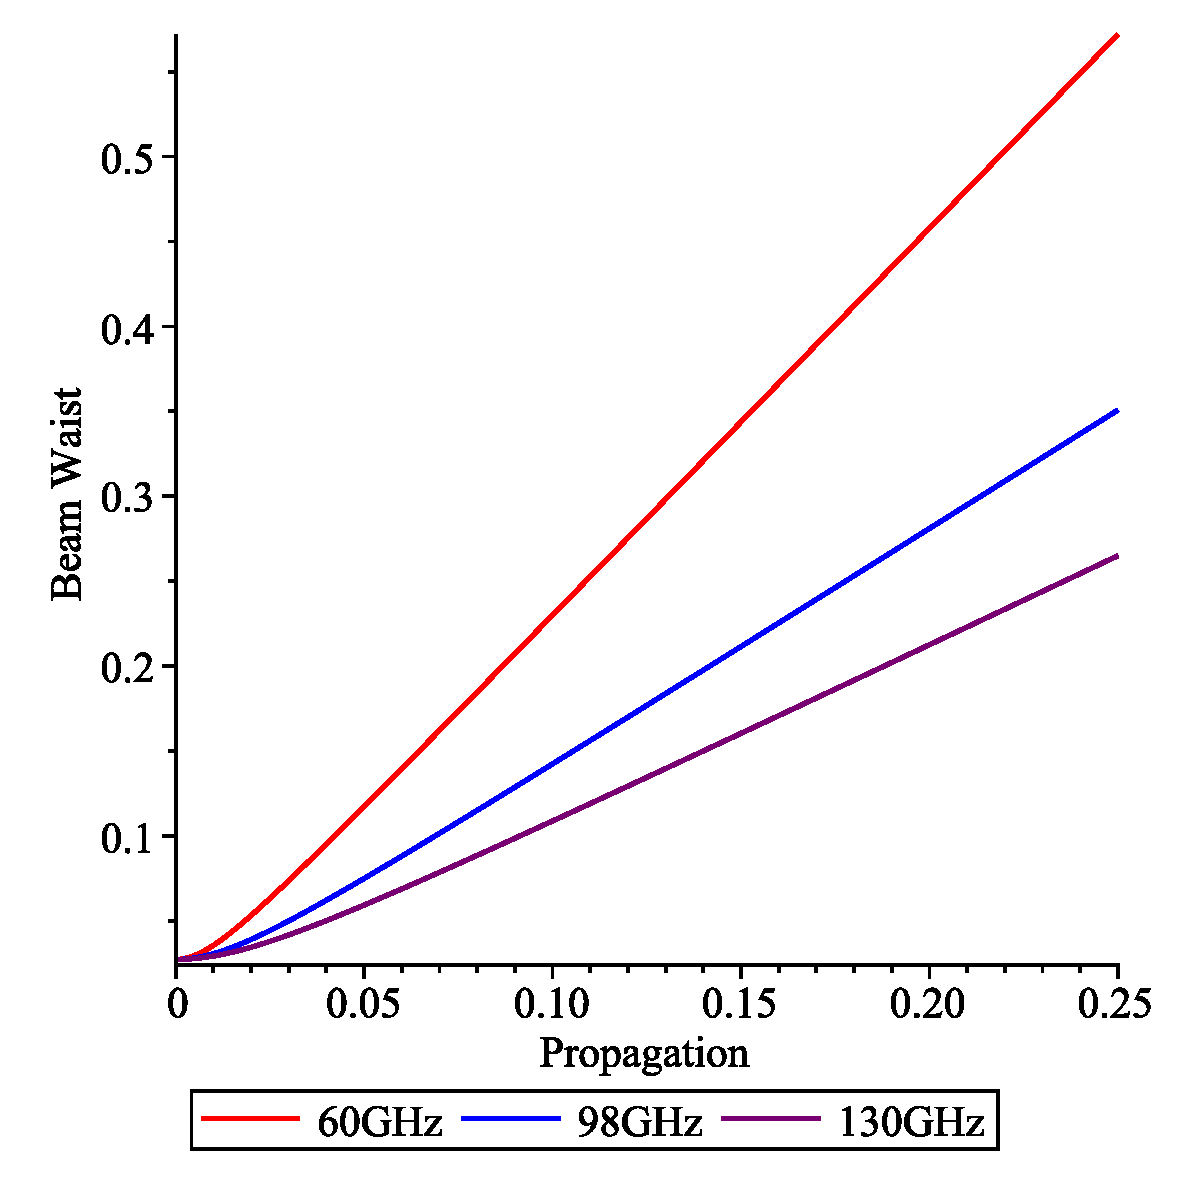
\includegraphics[width=\textwidth]{Figures/BeamProp.eps}
	\end{columns}
\end{frame}
\begin{frame}{Phaseshifts}
	\centering
	\begin{table}
		\begin{tabular}{lrr}

			Frequency \(\bqty{\si{\giga\hertz}}\) & \multicolumn{2}{c}{Phase at\(\bqty{2\pi}\)}                                                 \\
			                                      & \(n_e=\SI{10e16}{\per\meter\cubed}\)        & Phase at \(n_e=\SI{10e18}{\per\meter\cubed}\) \\
			2.45                                  & 0.8620                                      & 86.17                                         \\
			60                                    & 0.0352                                      & 3.519                                         \\
			98                                    & 0.0215                                      & 2.154                                         \\
			130                                   & 0.0162                                      & 1.624                                         \\
		\end{tabular}
	\end{table}
\end{frame}
\begin{frame}{Gaussian Telescope}
	\begin{columns}
		\column{.6\textwidth}
		\begin{itemize}
			\item Input parameters:\\
			\(w_0\), \(freq\), \(d_0\), \(f_0\), \(f_1\)
			\item Output distances:\\
			\(d_1 = 0.1619\), \(d_2 = 0.0881\), \(d_3 = 0.0563\)
			\item Output beamwaists:\\
			\(w_1 = 0.0116\), \(w_2 = 0.0069\)
			\item Wavelenght: \(\lambda=0.005\)
		\end{itemize}
		\column{.7\textwidth}
		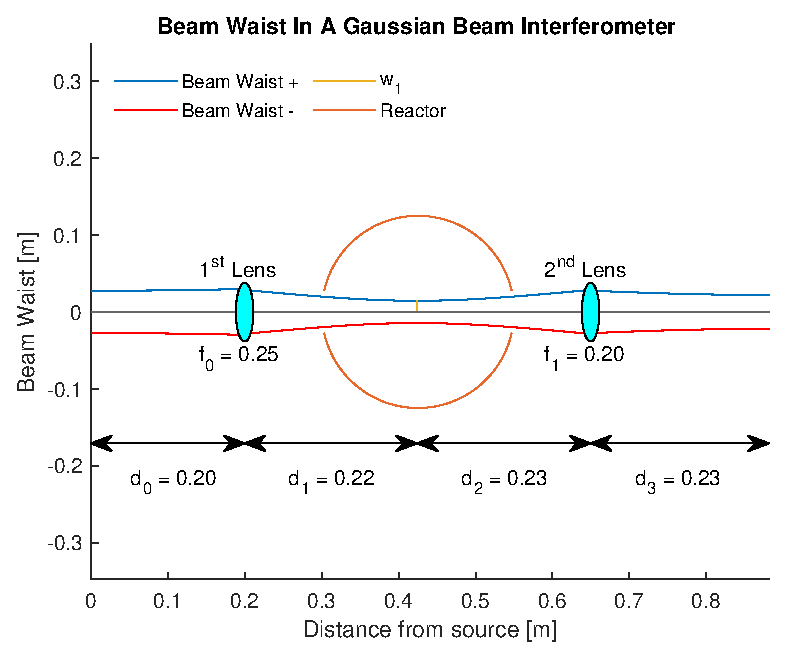
\includegraphics[width=\textwidth]{MatlabFigures/Interferometer/Interferometer.eps}
	\end{columns}
\end{frame}
\section*{Questions}
\title{Questions}
\subtitle{}
\begin{frame}
	\titlepage
\end{frame}

\end{document}
